
There are many additional factors which influence the users perception of a tag cloud, these must be taken into consideration on application of a tag cloud metaphor to data.

\begin{itemize}
	\item Tag length
	\item Number of characters
	\item White space
	\item Position within cloud
	\item Tag area
	\item Proximity effect
	\item Clustering
	\item Layout - spiral, typewriter
\end{itemize}

 %*Inter-dependencies *
 %*Known effects and possible research questions *
There are also specific requirements for tag cloud visualisation of software engineering data, which must be taken into account. These include issues of scale, the displaying of relationships, long identifiers and multiple word tags. There are very few existing tag cloud implementations which support visualisation of software engineering data. One such implementation is the Sonar Software Analysis Platform\footnote{http://www.sonarsource.org} which includes a tag cloud component which can be used to visualise various calculated software metrics. See Figure \ref{fig:sonarcloud} for an example of a Sonar visualisation of open source software project `Aspectj', containing 2,342 classes. Issues of both scale and long identifiers are apparent.  

\begin{figure}[h!]
	\centering
	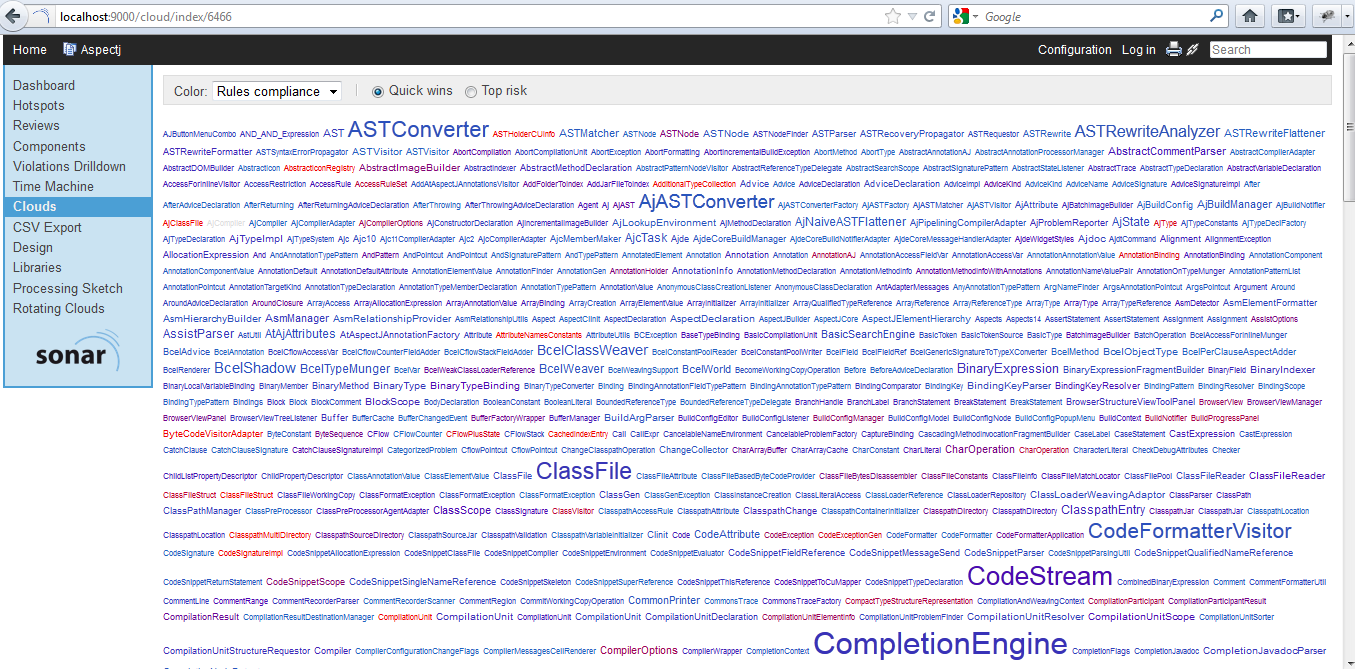
\includegraphics[scale=0.35]{sonarcloud.png}
	\caption{Aspectj visualised in Sonar Software Analysis Platform}
	\label{fig:sonarcloud}
\end{figure}

% ------------------------------------------------------------------------

%%% Local Variables: 
%%% mode: latex
%%% TeX-master: "../thesis"
%%% End: 
